\documentclass[oneside,12pt]{report}  

% the dimensions of the page
\textheight=9.25in \topmargin=-0.5in   %See note in Chapter 8 of Sample Report about "Page scaling" option in Adobe
\textwidth=6.0in
\oddsidemargin=0.3in
\evensidemargin=0.3in  % Needed to balance even and odd pages in twoside print copy


% Useful packages
\usepackage{dtklogos}
\usepackage{amsmath}
\usepackage{bm}
%\usepackage[colorlinks=true,pagebackref,linkcolor=blue]{hyperref}
\usepackage{amsfonts}
\usepackage{amsthm}
\usepackage{amsmath}
\usepackage{algorithm}
\usepackage{algorithmic}
\usepackage{graphicx, subfigure}
\usepackage{caption}
\usepackage{excludeonly}

\usepackage{graphicx} 

%\usepackage{doc}
%% Following sets up logic and formatting for conditional twoside copying
%\usepackage{ifthen, color, fancyvrb}
%\usepackage{nextpage}\pagestyle{plain}
%\newcommand\myclearpage{\cleartooddpage
%  [\thispagestyle{empty}]
%  }

\graphicspath{{./pictures/}}

\DeclareMathOperator*{\argmin}{arg\ min}
\DeclareMathOperator*{\sign}{sign}

% Note special alternative codes for using TWO bibliographies; see cautionary note in
\DeclareGraphicsExtensions{ps,eps,PNG,png}

% Theorem-like command definitions:
\newtheorem{theorem}{Theorem}[chapter]
\newtheorem{lemma}{Lemma}[chapter]
\newtheorem{definition}{Definition}  % Note, this italicizes everything

% Print the chapter and sections in the toc
\setcounter{tocdepth}{1}

% Specify which files to typeset for this run (note that overall pagination is preserved)
%\includeonly{chapter1, chapter2}
% Specify which files NOT to typeset for this run (note that overall pagination is preserved)
%\excludeonly{}

% Groundwork for allowing double-sided copying with blank versos
\def\prefacesection#1{
\chapter*{#1}
\addcontentsline{toc}{chapter}{#1}
}

\begin{document}


\def\thefootnote{\fnsymbol{footnote}}

\thispagestyle{empty}

% The numbers below controls the amount of space between the following sections
\def\shiftdowna{0.32in}  % Adjust for balance
\def\shiftdownb{0.22in}  % Adjust for balance

% Set up the boiler plate at the top of the page

\begin{center}
\textbf{{\large Mathematical Modeling and Consulting }}\\

\vspace \shiftdowna

\includegraphics[width=0.5\textwidth]{jhu.png}\\

% Home Department
\vspace \shiftdowna
\underline {Sponsor}\\ 
\vspace{5pt}
\textbf{\large The RAND Corporation} \\
\vspace\shiftdowna
\textbf{{Progress Report}}

% TITLE
\vspace \shiftdowna
\textbf{{\Large Large Graphical Models to Explore the Effects of Globalization and Development on Prevalence of Obesity}}

% STUDENTS
\vspace{0.35in}
\underline {Team Members}\\

Michael Weinberger, \texttt{michael.lee.weinberger@gmail.com} \\
\vspace{3pt}
\text{Zhendan Zhu}, \texttt{zhendanzhu@hotmail.com} \\
\vspace{3pt}
\text{Shannon Cebron}, \texttt{scebron@cis.jhu.edu}

% INSTRUCTOR
\vspace \shiftdownb
\underline {Academic Mentor} \\
\vspace{5pt}
\text{Dr.~N.~.H.~Lee}, Applied Mathematics and Statistics\\
\texttt{nhlee@jhu.edu}

% Consultants
%\vspace \shiftdownb 
%\underline {Consultant}\\
%\vspace{5pt}
%Jason Bourne\\

% DATE
\vspace \shiftdowna
Date: Last Compiled on \today

\end{center}

\vfill  %Fill page to force following note to bottom
\footnoterule
\noindent \small{This project was supported by Johns Hopkins University.}

% Begin ABSTRACT
\ifthenelse{\boolean{@twoside}}{\myclearpage}{}
\prefacesection{Abstract}

In recent years, obesity has become a global epidemic, affecting not only citizens of first-world countries, but also citizens of those countries experiencing rapid trade development. The link between globalization and obesity has been explored by some organizations, but not in a rigorous mathematical context. This project seeks to develop a mathematical description of this uptake in obesity, utilizing graphical constructs based in known information about countries’ development rates and trading habits, and using properties of these graphs to build regression models which can accurately predict obesity rates.

% Begin ACKNOWLEDGMENTS
%\ifthenelse{\boolean{@twoside}}{\myclearpage}{}
%\prefacesection{Acknowledgments}

% Table of contents, List of Figures, and List of Tables.
\ifthenelse{\boolean{@twoside}}{\myclearpage}{}
\tableofcontents

%\ifthenelse{\boolean{@twoside}}{\myclearpage}{}
%\listoffigures

%\ifthenelse{\boolean{@twoside}}{\myclearpage}{}
%\listoftables


\renewcommand{\thefootnote}{\arabic{footnote}}
\setcounter{footnote}{0}

\ifthenelse{\boolean{@twoside}}{\myclearpage}{}
%\include{A_Introduction}
%\include{B_TechnicalBackground}
%\include{C_ProblemStatement}
%\include{D_Analysis}
%\include{E_Results}
%\include{F_Conclusion}

%\include{chapter1}
%\include{chapter2}
%\include{chapter3}
%\include{chapter4}
%\include{chapter5}
%\include{chapter6}

\chapter{Introduction}

Obesity is a medical condition identified by a Body Mass Index (BMI) (an adjusted proportion between height and weight) greater than 30. Obesity is proven to have extreme effects on a person`s quality of life \cite{health}. It is a major predictor in several potentially deadly types of disease; a common cause of physical degradation in the body manifested through pain in the joints and difficulty walking and moving; an aggravator of existing conditions such as sleep apnea and acid reflux disease; and a known detriment to mental health for reasons of body image and self-confidence.

When present in large proportions in populations, obesity is a major public health problem and a leading cause of preventable death. Treatment for heart disease, asthma, and diabetes is costly, driving up the cost of health care for the whole population. Furthermore, lost work hours due to obesity-related health problems detract from the health of the local economy.

As of 2010, the United States Center for Disease Control reports that 35.7 percent of the American population is obese, and this number has been steadily increasing since the 1960s \cite{prevalence}. The federal government estimates that up to USD 117 billion is lost yearly due to direct and indirect costs of such an obese population \cite{prevalence}.

The prevalence of obesity is increasing in countries around the world, at the highest rates in countries recently achieving highly developed status as according to the Human Development Index (a weighted average exceeding 0.8 between measures of education, life expectancy, and personal wealth). However, in some countries this effect is more pronounced than in others, and at this level of detail, the spread of obesity is not well-understood. It is surmised that through increased trade and increased personal disposable income, more processed food has become available around the world. Furthermore, rapid changes in technology have allowed nations to become more culturally integrated with one another, and some experts suggest that citizens of developing countries are becoming more and more influenced by the dietary and exercise habits of their developed neighbors.

A better understanding of the interplay between development, globalization, and obesity may contribute positively to efforts to prevent the spread of this preventable, expensive, and deadly disease.

The RAND Corporation is a public policy thinktank which conducts research and analysis to support political decision-making and the public good. Many elected persons agree that legislation may help to curb the obesity epidemic, and it is important that this legislation is designed in an informed, rigorous manner. By working with the RAND Corporation to conduct this project, we can help to give lawmakers insight into what factors most prominently affect obesity trends.

\chapter{Technical Background}

\section*{Regression Analysis}

Regression analysis is a statistical technique for estimating the relationships between different variables. A standard regression model consists of a single response, or dependent variable; and one or more predictor, or independent variables. The purpose of such a model is to predict how changes in these independent variables elicit changes in the response variable.

More specifically, a regression model relates the response variable, \begin{math}Y\end{math}, to a function of the vector of independent variables, \begin{math}X\end{math}, and their corresponding coefficients vector, \begin{math}\beta\end{math}. The prediction function has the form \begin{math}\hat{Y} = f(X,\beta) + \epsilon\end{math}.

Several underlying assumptions come with performing regression analysis. First, we must assume that the sample we are using is representative of the population for which the inference will be useful. Since our sample data consists of nearly every country, our model meets this assumption. Second, we must assume that the errors for each prediction instance are independent from one another and from the value of the independent variables - more specifically, \begin{math}E[\varepsilon_i|x_i] = E[\varepsilon_i] = 0\end{math}. We can control for meeting this assumption by examining data on the residuals of our model - the differences between the predicted values and actual values for each instance. If the assumption is met, then these residuals will follow no particular pattern, appearing to be random and uncorrelated with any other factors.

Third, we assume that the predictors are not correlated with one another; that is, no two independent variables are telling us the same information and thus clouding the quality of our model. We can control for this by investigating a covariance matrix among all independence variables, and taking action to modify, combine, or remove such variables that have a high correlation with another variable. The current standard is that a correlation value between two independent variables of 0.4 or greater warrants further investigation. Variables with a correlation value of 0.8 or greater are almost certainly causing multicollinearity in the model. The consequences of this situation are that the affected coefficients have larger standard errors than they otherwise would - our estimates are less precise; the model tends to overfit the data; and some computer programs may produce numerically inaccurate estimates because the matrix \begin{math}X^{T}X\end{math} is either not invertible, or not invertible at the level of accuracy that the software has. Some standard remedies for the problem of multicollinearity include dropping one of the variables, mean-centering the variables, or creating a new variable which represents both variables together.

Finally and most importantly, for a linear regression model, it is assumed that each predictor variable has a linear relationship with the response variable, which in our case, is obesity. Some variables may appear to have logarithmic, exponential, polynomial, or even more complicated relationships with the response variable. There are standard variable transformations to deal with these more complicated relationships and manifest them as linear ones. For example, if it appears that the obesity rate varies closely with the square root of a variable, then we transform that variable into its square root for inclusion in our regression analysis. This new variable can be equally informative to the original version, while also meeting the assumptions demanded by the regression model.

Alternatives to a linear regression model existed. More specifically, with the tools available, we had the opportunity to choose between linear regression, Gaussian regression, logit regression, Poisson regression, Gamma regression, inverse Gaussian regression, and quasipoisson regression. However, the other types of regression in this list assume a different structure of the data and a different presumed relationship between the independent variables. For example, Poisson regression deals with counting data, and expected counts based on certain factors. Estimating the count of obese people in a country is not an appropriate regression task because our data do not meet the assumptions of a Poisson model. Quasipoisson regression is a modified form of this. Gaussian and inverse Gaussian regression concern estimates of functions that must pass through specific sets of points. Logit regression estimates the odds of an outcome, essentially acting as a binary classification model. Gamma regression is a more generalized form of Poisson regression. None of these types of regression except linear are an appropriate fit for our data and goal.

For multiple linear regression, estimates for B are obtained through maximum likelihood estimation, which serves to find the set of coefficients B that minimizes the sum of squared differences between the actual and predicted values. Minimizing squared differences rather than absolute differences allows us to penalize progressively more those observations for which the prediction error is very large. More specifically, in utilizing maximum likelihood estimation, we give a function which gives the probability that the obesity rates are equal to their current values, given that the set of coefficients is B. The goal is to maximize this likelihood, which implies the greatest possible accuracy. We do so by taking the derivative of this function and solving for B when the function is equal to 0.

In the opposite of the case when two variables give us redundant information, it is also possible that two variables jointly give us more information then they do individually. In this case, we include an interaction term in our regression model, where the variables multiplied together is considered an additional independent variable. A coefficient is also estimated for this interaction term, just as for any other term in the model. With so many variables present in our obesity model, it is easiest to use software to step through all of the possible interactions and find out which ones contribute significantly to the strength of the model.

In terms of the model's strength, there are a number of criteria which it must meet. We conduct an F-test on the regression model, which tests the hypothesis that the model fits the data well. A p-value of less than 0.05 will be sufficient in this case. We also conduct a T-test on each individual coefficient estimate, which tests the hypothesis that the coefficient is nonzero. If the T-test is significant, i.e., has a p-value of less than 0.05, then we have shown within reasonable doubt that there is a significant linear relationship between the predictor and the response. We are also concerned with the model's coefficient of determination, or R2 value. The R2 value gives an estimate of what percentage of the data's variability is accounted for by the regression model. The value can fall between 0 and 1, and we would seek out a value of at least 0.8.

Predictor variables which do not have a strong linear relationship with the response variable may add noise to the model and detract from its accuracy. In general, we desire a model that is as simple as possible. We can conduct ANOVA tests between nested models to see if the model with added terms (whether interaction terms or additional independent variables) is significantly stronger than the smaller model. If it is not, then we elect to use the simpler model that explains the data with the same efficacy. If the ANOVA test result has a p-value of less than 0.05 then we accept the larger model.

The final model that we will settle on will have low enough p-values in all of these criteria, and will by virtue of the ANOVA test be stronger than any of the simpler models that are possible. It will also meet the assumptions listed above which are inherent to the use of linear regression to describe relationships among data.

\section*{Theoretical Graphs}

In mathematics, graph theory is the study of graphs, which are structures consisting of a collection of nodes (vertices), and arcs (edges) which connect pairs of nodes. Graph theory is of specific interest to our project because it allows for an abstraction of the relationships between world nations into a mathematical form that can be analyzed rigorously. Our primary goal in incorporating theoretical graphs into our project is to gather data from these graphs that can be used as potential independent variables in our regression analysis. The independent variables we use must exist as attributes of a country, and thus in terms of graph theory, we will specifically be interested in those graph features which characterize specific vertices, as this can be transformed into an independent variable corresponding to a country represented by the vertex.

The vertex characterizations which are of particular interest to us are as follows (please see the glossary for further definitions):
\begin{itemize}
\item Vertex degree
\item Shortest path to a specific vertex; e.g., for each country, we calculate the length of a shortest path from its corresponding vertex to the vertex representing the United States
\begin{itemize}
\item A weighted shortest path finds the shortest sum of edge weights leading to the target vertex
\item An unweighted shortest path finds the shortest number of edges on a path to the target vertex
\end{itemize}
\item Membership in a cycle
\item Membership in a maximal clique
\item The condition of being a cut vertex
\item The condition of being the endpoint of a cut edge
\end{itemize}

All of those listed vertex attributes can be converted into continuous or factor variables for use as independent variables in our regression analysis. The specific graphical independent variables used in our analysis will be discussed in later sections.

\section*{Data and Software}

Vast amounts of data for nations and sovereign entities are available from the CIA World Factbook and the World Health Organization's (WHO) databases. The data can be downloaded from these sources in .csv files. THese .csv files can be imported into the R environment and merged so that a data frame is built with several different independent variables listed for each country. The CIA World Factbook and WHO refer to some countries by different names (e.g., the Republic of Korea and South Korea are the same country, but named differently by these sources). In order to merge the lists properly despite these naming conflicts, another table was generated which listed possible alternate names for each country, and referenced during the merging process to ensure that data for South Korea and the Republic of Korea, for example, was combined. As a convention, the name used by the CIA World Factbook was our default name.

The R environment is effective for statistics and data management, but does not have a robust package for creating the type of graphs discussed in the previous subsection. Python, however, does have such a feature. Therefore, the data from R must be converted into a .csv file again, which is easily done with a data frame by using the "write.csv" command in R. However, our data frame with different independent variables does not define country contingencies in any way - i.e., the data needed to define edges in our graphs. This information must be mined from a webpage and processed to remove commas, footnotes, and other extraneous text that the CIA has included in their notes. This was done in Microsoft Excel by pasting the contents of the webpage onto a spreadsheet and processing the cells using Excel formulas. This was then exported as a second .csv file and imported into Python along with the country names in order to create the graphs.

Python maintains a package called Pygraph which allows for relative ease with creation of graphs, and ease of data extraction, such as shortest path data (see the previous subsection). These data were easily arranged by country and exported back into R, for merging into our main data frame. After this step, we several dozen potential independent variables to consider in our regression analysis, when combining our initial 16 independent variables with another 20 independent variables that were extracted from our theoretical graphs. At this point we were ready to begin testing relationships and building regression models in R, based on the criteria explained above.

R also offers the opportunity for any user to create a package, which is a collection of R functions, data, and compiled code in a clearly-documented format. It is easy to include not only a developed regression model, accompanying data, and example code for diagnosing the model's strength or changing its parameters, but also to include images of our graphs, a glossary explaining independent variables in the model, a list of references, and more.

\chapter{Problem Statement}

	While large amounts of data on obesity exit, there is one problem. Even with the myriad of statistical tools that exist, there has yet to be research into the correlation between obesity and country development. With obesity rates continuing to rise, there needs to be a way to determine what causes this disease to grow and spread. Being able to determine how obesity is affected by globalization and cross cultural relations, will be beneficial to the world health community, and lead to a net benefit for the world’s population.

The RAND Corporation, among other policy making organizations, need help to make better informed decisions about obesity. To combat the increase in obesity rates and save lives, a solution to this problem must be discovered. Currently, these groups are just guessing about how to combat obesity, with no real data or information about what regulations would best help developing countries to cut back their obesity rates. While obesity is not yet been a catastrophic event, we believe that without help there may be irreversible damage to world health.

Using statistical analysis, our results provide insight into what is causing the great rise in obesity rates across the globe. We undertook the task of determining what variables are important in understanding those rates. Elements such as trading partners, cultural influence, and geographical distance for example, were all tested as predictors for obesity rates. In addition we will used graphical elements and algorithms, to build graphs of these factors, such as difference in obesity rates between two countries, and then ran algorithms such as shortest path, to extract information about obesity across distances.

With our results in mind, these organizations will have a tool that allows them to directly attack the problem, giving them a better solution and the ability to pass valuable restrictions.

\chapter{Analysis}

\section*{Non-graphical independent variables}

The following independent, non-graphical variables were investigated during our model building:
\begin{itemize}
\item Total electricity consumption
\item Fertility rate
\item Youth unemployment
\item Total population
\item Per person imports (USD)
\item Per person GDP (USD)
\item Percentage of children under age 5 who are underweight
\item Population growth rate
\item Birth rate
\item Education expenditures as a percentage of GDP
\item Health expenditures as a percentage of GDP
\item Inflation rate
\item Gini index for families
\item Total internet users
\end{itemize}

Relationships individually between these independent variables and the response variable, obesity rate, were explored for inclusion in a regression model. For the following variables, we were unable to find a linear relationship, or find a suitable transformation to elicit a linear relationship:

\begin{itemize}
\item Electricity consumption
\item Youth unemployment
\item Education expenditures as a percentage of GDP
\item Health expenditures as a percentage of GDP
\item Inflation rate
\item Gini index
\item Total internet users
\end{itemize}

These variables were removed from consideration in regression analysis.

\begin{figure}
\centering
\caption{Example scatterplot of a lack of linear relationship, between inflation rate and obesity rate (the overlaid line is the simple regression line)}
\label{fig:inflation-obesity-scatter}
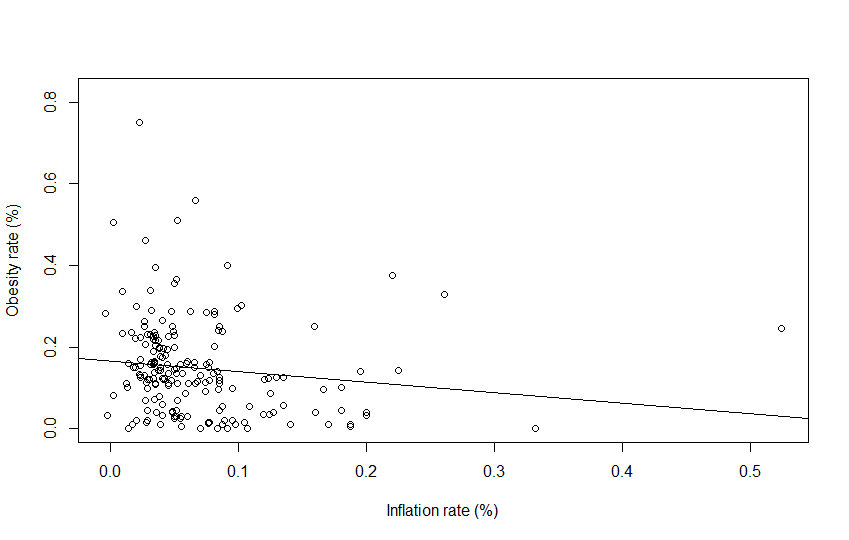
\includegraphics[width=\textwidth]{inflation-obrate-scatter.png}
\end{figure}

The following are those variables which had a significant linear relationship, without any linearizing transformations required. They are listed along with the p-value from the T-test used to test the strength of the relationship.

%should we have some plots along with this list to illustrate the relationships?
\begin{itemize}
\item Fertility rate (\begin{math}p=6.35\cdot10^{-07}\end{math})
\item Total population (\begin{math}p=0.0521\end{math})
\item Per person GDP (USD) (\begin{math}p=0.00525\end{math})
\item Percentage of children under age 5 who are underweight (\begin{math}p=5.05\cdot10^{-15}\end{math})
\item Population growth rate (\begin{math}p=1.60\cdot10^{-06}\end{math})
\item Birth rate (\begin{math}p=1.43\cdot10^{-06}\end{math})
\end{itemize}

\begin{figure}
\centering
\caption{Example scatterplot of a strong linear relationship, between fertility rate and obesity rate (the overlaid line is the simple regression line)}
\label{fig:fertility-obesity-scatter}
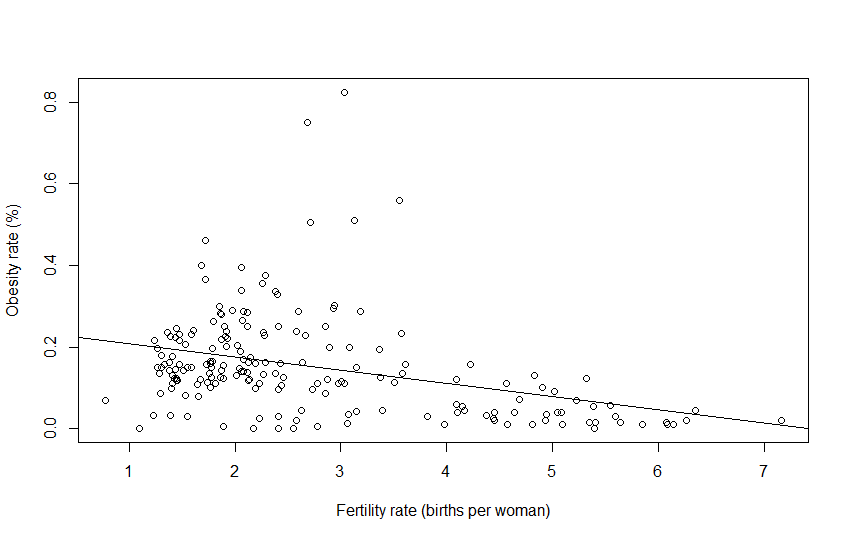
\includegraphics[width=\textwidth]{fertility-obesity-scatter.png}
\end{figure}

Finally, some variables showed a stronger linear relationship following a transformation of some kind. This group of variables is also listed along with their transformations and their T-test p-values.

%should we show some plots of before and after?
\begin{itemize}
\item Per person imports (USD)
	\begin{itemize}
	\item Transformation: \begin{math}f(x) =\log{x}\end{math}
	\item \begin{math}p=2.70\cdot10^{-07}\end{math}
	\end{itemize}
\item Per person GDP (USD)
	\begin{itemize}
	\item Transformation: \begin{math}f(x) = \log{x}\end{math}
	\item \begin{math}p=1.85\cdot10^{-07}\end{math}
	\end{itemize}
\item Percentage of children under age 5 who are underweight
	\begin{itemize}
	\item Transformation: \begin{math}f(x) = \sqrt{x}\end{math}
	\item \begin{math}p=2.00\cdot10^{-16}\end{math}
	\end{itemize}
\end{itemize}

\begin{figure}
\centering
\caption{Plots of per person imports versus obesity rate, before and after the linearizing transformation (regression lines overlaid)}
\label{fig:ppimports-obesity-prepost}
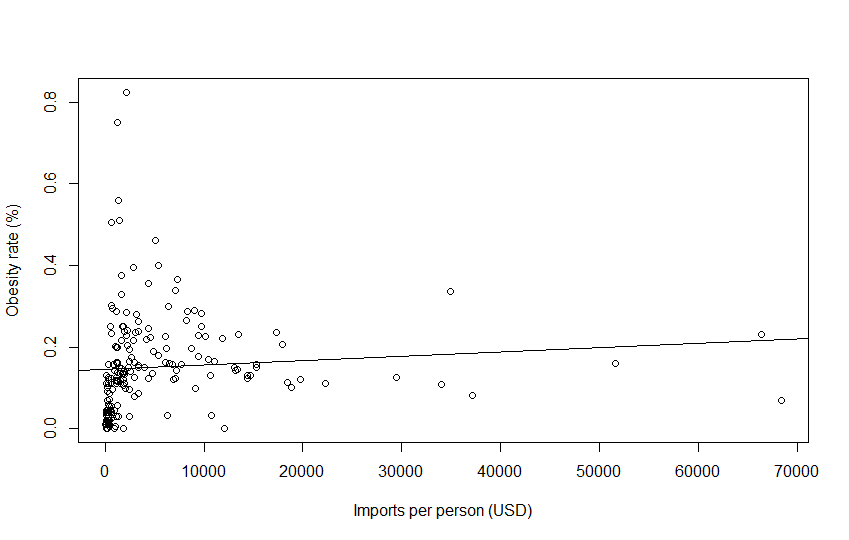
\includegraphics[width=\textwidth]{ppimports-obesity-pretransform.png}
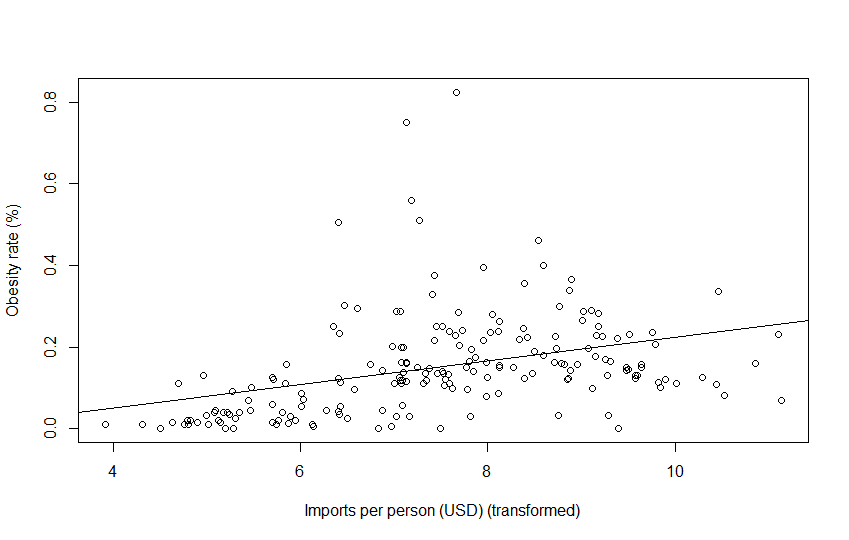
\includegraphics[width=\textwidth]{ppimports-obrate-posttransform.png}
\end{figure}

\section*{Choice of graphs and graphical independent variables}

The following variables were extracted from our graphs in Python :
\begin{itemize}
\item From the undirected graph of border relationships (hereafter, Graph 1):
	\begin{itemize}
	\item Shortest path to the United States in terms of number of edges
	\item Shortest path to the United States in terms of sum of edge weights, defined by border length in kilometers
	\end{itemize}
\item From the directed graph of import relationships:
	\begin{itemize}
	\item Number of incoming edges (i.e., the number of countries which have that country as a major source of imports)
	\item TO BE CONTINUED
	\end{itemize}
\item From the directed graph of export relationships:
	\begin{itemize}
	\item Number of outgoing edges (i.e., the number of countries which import a major amount from that country)
	\item TO BE CONTINUED
	\end{itemize}
\end{itemize}

%%%%begin copied section

Relationships individually between these graph-extracted independent variables and the response variable, obesity rate, were also explored for inclusion in a regression model. For the following variables, we were unable to find a linear relationship, or find a suitable transformation to elicit a linear relationship:

\begin{itemize}
\item TO BE CONTINUED
\end{itemize}

These variables were removed from consideration in regression analysis.

The following are those variables which had a significant linear relationship, without any linearizing transformations required. They are listed along with the p-value from the T-test used to test the strength of the relationship.

\begin{itemize}
\item \emph{Graph 1}: Shortest path to the United States in terms of number of edges (\begin{math}p=1.48\cdot10^{-05}\end{math})
\item \emph{Graph 1}: Shortest path to the United States in terms of sum of edge weights, defined by border length in kilometers (\begin{math}p=4.48\cdot10^{-08}\end{math})
\end{itemize}

\begin{figure}
\centering
\caption{Example scatterplot of a strong linear relationship, between shortest path to the United States and obesity rate (the overlaid line is the simple regression line)}
\label{fig:shortpath-obesity-scatter}
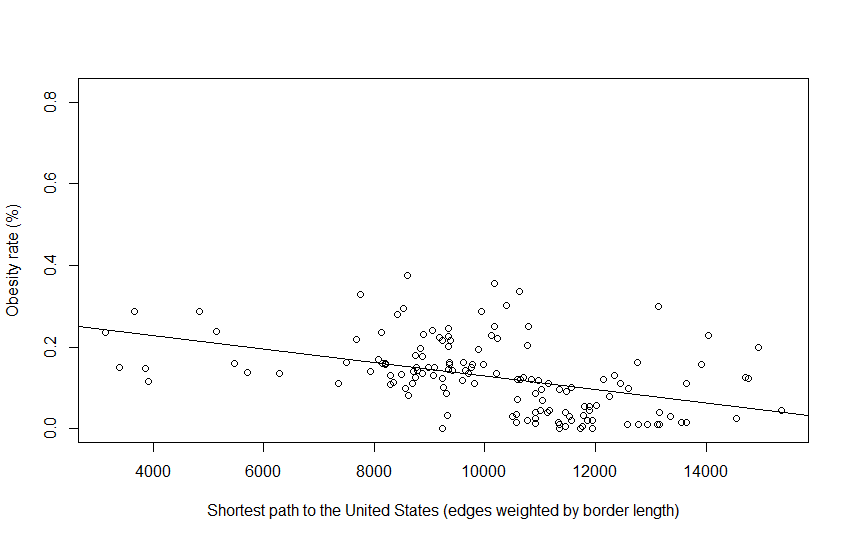
\includegraphics[width=\textwidth]{borderdegrees_wtd-obrate-scatter.png}
\end{figure}

Finally, some variables showed a stronger linear relationship following a transformation of some kind. This group of variables is also listed along with their transformations and their T-test p-values.

%should we show some plots of before and after?
\begin{itemize}
\item TO BE CONTINUED
	\begin{itemize}
	\item Transformation:
	\item
	\end{itemize}
\end{itemize}

\begin{figure}
\centering
\caption{Plots of per person imports versus obesity rate, before and after the linearizing transformation (regression lines overlaid)}
\label{fig:ppimports-obesity-prepost}
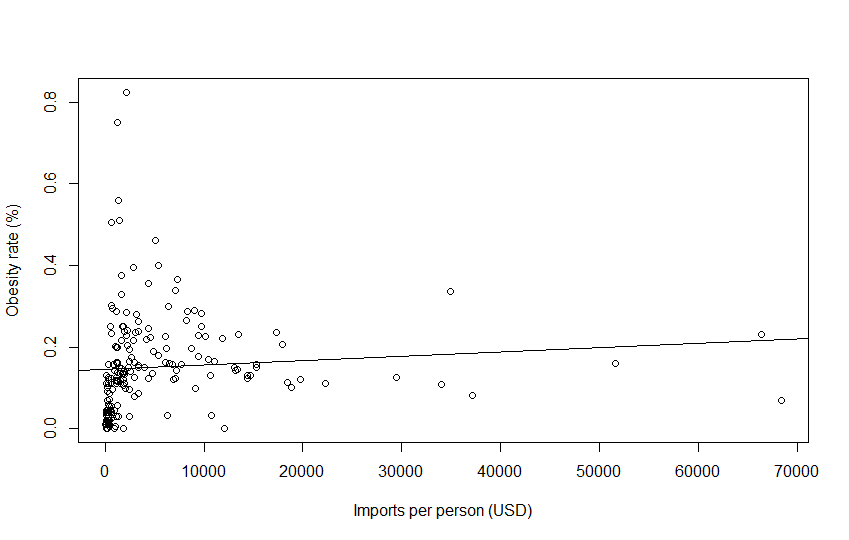
\includegraphics[width=\textwidth]{ppimports-obesity-pretransform.png}
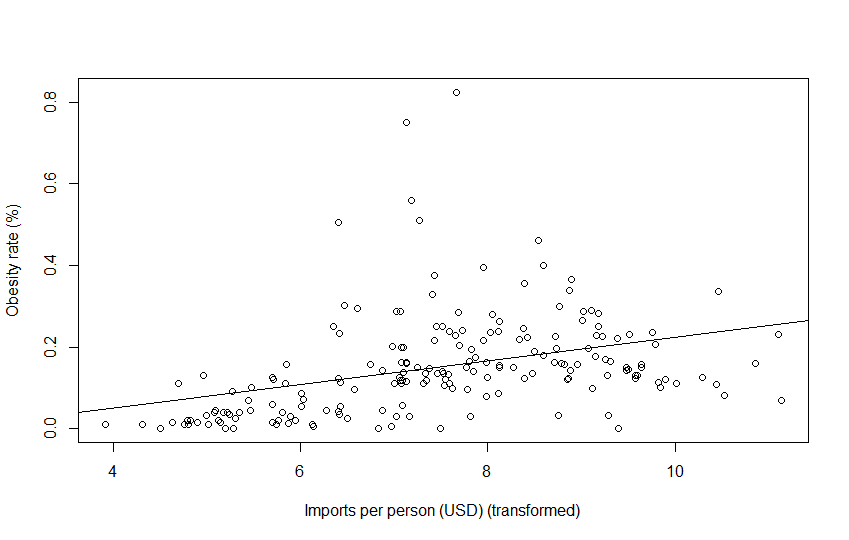
\includegraphics[width=\textwidth]{ppimports-obrate-posttransform.png}
\end{figure}

%%%%end copied section

\section*{Relationships among independent variables}
\subsection*{Multicollinearity}

We calculated correlation values between all pairs of independent variables as a check for the effect of multicollinearity on our model. The correlation between fertility rate and birth rate was \begin{math}0.9703\end{math}, compared to a maximum value of \begin{math}1\end{math}. The relationship between the two is evident from a scatterplot. 

\begin{figure}
\centering
\caption{Scatterplot of fertility versus birth rate, overlaid with a simple regression line}
\label{fig:fertility-birth_rate}
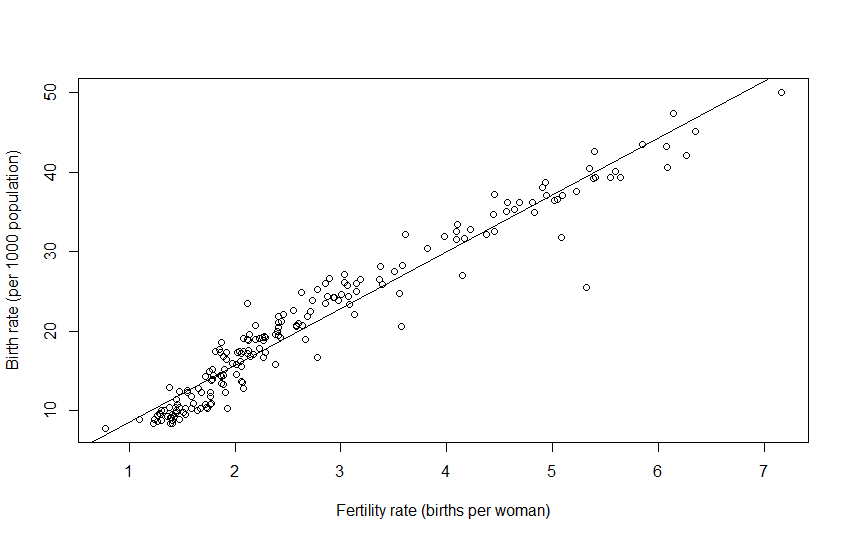
\includegraphics[width=\textwidth]{fertility-birth_rate.png}
\end{figure}

As discussed in the previous chapter, this relationship, known as multicollinearity, means that the two variables are offering redundant information to our model. For this particular case we were able to find an easy solution. We created a new independent variable equal to the fertility rate multiplied by the birth rate. A hypothesis test on the linear relationship of this new variable with obesity rate gave \begin{math}p=3.29\cdot10^{-08}\end{math}, which is even smaller than the p-values for the variables individually.

\begin{figure}
\centering
\caption{Scatterplot of the new variable versus obesity, overlaid with a simple regression line}
\label{fig:fertility.birth_rate}
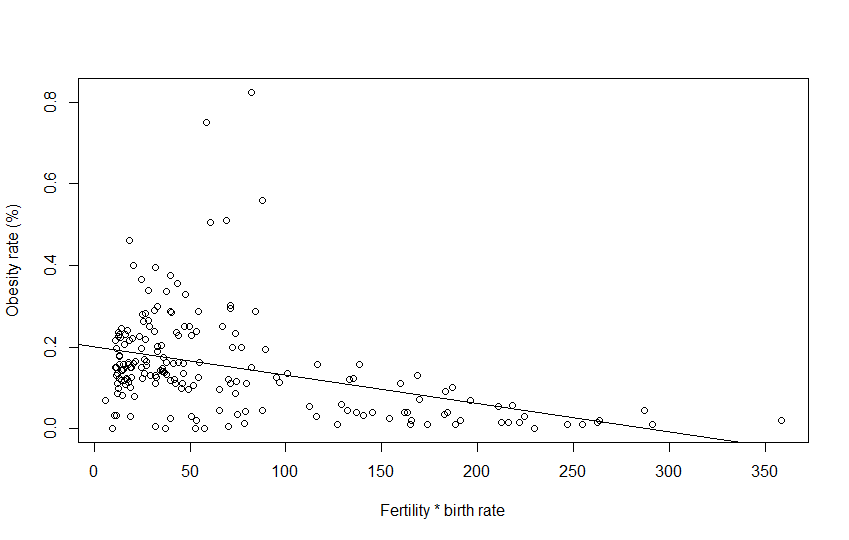
\includegraphics[width=\textwidth]{fertility-birth_rate-obesity-scatter.png}
\end{figure}

There was also a very strong correlation between the two variables extracted from Graph 1, shortest path to the United States in terms of number of edges, and in terms of sum of edge lengths when weighted by national border length. These two variables had a correlation of \begin{math}0.9050\end{math}. In this situation, we did not find that combining the two variables into a new variable was able to yield a stronger relationship than the variables on their own. Therefore, we dropped from our analysis the variable which had a weaker linear relationship with obesity rate, which was the shortest path in terms of the number of edges.

\section*{Stepwise regression to determine final variable inclusion}

Talk about which variables were significant at first but then later got eliminated because in the multiple model they weren't significant

\section*{Validation of usage of graphical variables}
ANOVA test used to show that the model with the graphical variables is more informative than the model without them (TO BE CONTINUED)

\chapter{Results}

After analyzing all of the potential independent variables, checking for linear regression assumptions, and verifying the significance of all relevant hypothesis tests and statistics, we developed a final regression model:
\\
\\
\begin{math}
\hat{Y} = f(X,\beta) + \epsilon
\end{math}
\\
\\
where
\\
\begin{math} X = 
\begin{pmatrix}
x1 \\ x2 \\ \sqrt{x3} \\ x4 \\ \log{x5}
\end{pmatrix}
\end{math}
\\
and
\begin{math} \beta =
\begin{pmatrix}
0.01 \\ -0.045 \\ 56 \\ 1.23\cdot10^{-3}
\end{pmatrix}
\end{math}
\\ \\
In the appendix, a final list of variables corresponding to the vector X and detailed explanations of their meanings can be found.

\begin{math} \rho =
\begin{pmatrix}
p(x_1) \\ p(x_2) \\ \vdots \\p(x_{27})
\end{pmatrix}
\end{math}

where \begin{math}p(x_i)\end{math} is the p-value resulting from the hypothesis test that the slope coefficient is zero versus the hypothesis that it is nonzero

\chapter{Conclusion}

-Explain meaning of model in terms of what the variables actually represent
\\
-Talk about remaining deficiencies with the model and how they could be improved in the feature, such as the problem of missing information for some predictors
\\
-Talk about other possibilities for future research

\ifthenelse{\boolean{@twoside}}{\myclearpage}{}

\appendix
\ifthenelse{\boolean{@twoside}}{\myclearpage}{}

%\chapter{Lemmas}\label{Lemma}

\chapter{Glossary}\label{Glossary}

\vspace{12pt}

\vspace{8pt}
\noindent {\bf Obesity}. A medical condition that Body Mass Index is greater than 30.

\vspace{8pt}
\noindent {\bf Body Mess Index}. Body Mass Index is defined as the individual's body mass divided by the square of his or her height.

\vspace{8pt}
\noindent {\bf Vertex-edge graph}. A set of vertices (also called nodes), along with a set of edges (also called arcs), in which each edge must correspond to two vertices as its endpoints. The edge may or may not have direction. A simple graph is one that does not allow multiple edges between the same two vertices, or an edge that has the same vertex as both of its endpoints.

\vspace{8pt}
\noindent {\bf Human Development Index}. A composite statistic of life expectancy, education, and income indices to rank countries into four tiers of human development.

\vspace{8pt} \noindent {\bf Vertex degree}. In graph theory, the degree (or valency) of a vertex of a graph is the number of edges incident to the vertex, with loops counted twice..

\vspace{8pt} \noindent {\bf Clique}. In graph theory, a clique is a subset of a graph's vertices such that every two vertices in the subset are connected by an edge.

\vspace{8pt} \noindent {\bf Regression}. Regression is a method for modeling the relationship between a single response variable and one or more independent variables which are thought to have a relationship with the response variable. If this relationship is linear, then it is linear regression. If the response variable comes from a finite set of outcomes, then we use logistic regression, which calculates the odds of the response variable taking on each outcome. Coefficients are estimated for each independent variable such that the deviation between actual and predicted values is minimized.

\vspace{8pt} \noindent {\bf Residuals}. In regression analysis, a regression model's residuals are the squared distances between actual values of the response variable and the the values predicted by the model. Generally, if the residual values appear to follow a pattern, rather than being randomly dispersed, we might surmise that the current model is not an appropriate choice for modeling the data.

\vspace{8pt} \noindent {\bf Hypothesis test}. A hypothesis test compares a null hypothesis to an alternative hypothesis. The null hypothesis is rejected if, under the assumption that it is true, the probability of observing the true data is less than a specified significance value. In the statistics community it is standard to use 0.05 as this value.

\vspace{8pt} \noindent {\bf Gini index}. A probabalistic measure of dispersion of incomes in a society, where a higher Gini index indicates more income inequality - i.e., a bigger gap between rich and poor.

\vspace{8pt} \noindent {\bf .csv file}. A file that stores tabular data in plaintext format, and can be easily processed in most programming languages. Rows are separated by line breaks, and row entries are separated by commas, tabs, semicolons, or other user-specified delimiters.


\ifthenelse{\boolean{@twoside}}{\myclearpage}{}
\chapter{Acronyms}\label{Acronyms}

\noindent {\bf CIA} Central Intelligience Agency
\vspace{5pt}

\noindent {\bf GDP} Gross Domestic Production

\vspace{5pt}

\noindent {\bf BMI} Body Mass Index

\vspace{5pt}

\noindent {\bf WHO} World Health Organization

\vspace{5pt}

\noindent {\bf CSV} Comma-separated Values

\vspace{5pt}

\noindent {\bf USD} United States Dollars

%\endinput

% Add your bibliography to Contents
\ifthenelse{\boolean{@twoside}}{\myclearpage}{\newpage}
\addtocontents {toc}{\protect \contentsline {chapter}{REFERENCES}{}}
\addcontentsline{toc}{chapter}{Selected Bibliography Including Cited Works}  

% Bibliography must come last.
\bibliographystyle{plain}
\renewcommand\bibname{Selected Bibliography Including Cited Works}
\nocite{*}  % List ALL references in your references, not just the ones cited in the text.
% This scheme automatically alphabetizes the Bibliography.
\bibliography{Biblio}
\end{document}
